%%% Copyright 2004 by Till Tantau <tantau@users.sourceforge.net>.
%%% Modified by Ken Wilder. Modified again by Winnie van Dijk.
%%% The original can be found in the beamer distribution.
%%% Used with permission.

\documentclass{beamer}

%%% Set the theme
\usepackage{style/wvd_beamertheme_lecture}
\usepackage{tikz}
\usepackage{tikz-qtree}
\usetikzlibrary{trees}


%%% View lists in a stepwise fashion, not all at once
%\beamerdefaultoverlayspecification{<+->}





%%% Define the title page elements
\title{Introduction to R for Economists}
\subtitle[Part 1]
	{Basic Programming Principles and Data Analysis (Part 1)
	}
\setcounter{lecture}{1} %This sets the counters for theorems, examples, etc.
% \author{}
% \institute[University of Chicago]
% 	{University of Chicago / Becker Friedman Institute}





\begin{document}

%%% Title frame
\begin{frame}
  \titlepage
\end{frame}

\note{notes}

%%% Outline frame
\begin{frame}
 \frametitle{Outline}
 \tableofcontents%[pausesections]
\end{frame}

\note{notes}




% INTENDED OUTLINE

%Part 1: Intro to R, Matlab \& LaTeX
%1.    Good programming practice
%2.    Recap of R
%3.    Intro to Matlab (mostly comparing Matlab syntax to R)
%4.    Latex (based on https://www.sharelatex.com/learn/Learn_LaTeX_in_30_minutes)

%Part 2: Selected topics in economic data with illustrations in R
%5.    Functional approximation (to illustrate optimization and plotting using ggplot)
%6.    Census data / APIs
%7.    Useful public data sets
%8.    Making maps with ggmap
%9.    Useful packages (maybe also creating your own packages)
%10.   Summarizing data using data.tables and the tidyverse 
%11.   Ggplot examples (cheat sheet)
%12.   Packages
%13.   Shiny
%14.   Knitr and R notebooks










%%% Main content

\section{Intro \& logistics}

\begin{frame}[allowframebreaks]
 \frametitle{Administration}

	\begin{itemize}
	\setlength{\itemsep}{\fill}
		\vfill
		\item
		Part 1 learning objectives: 
		\begin{itemize}
			\item
			Basic universal programming skills.
			\item
			Getting started with RStudio and coding in the R language.
			\begin{itemize}
				\item
				Using the command line, defining variables, importing data, plotting, matrix operations, saving and running your code, regressions...
			\end{itemize}
			\item
			Some tips \& tricks for your econ homework, RA work, and future research projects.
		\end{itemize}
		\vfill
		\item
		Required software:
		\begin{columns}[t]
		\begin{column}{0.1\textwidth}
		\end{column}
		\begin{column}{0.8\textwidth}
		\begin{itemize}
			\item[R and RStudio]
			\vskip-.5cm
			Can be downloaded free of charge from \scriptsize\url{http://www.rstudio.com/}
		\end{itemize}
		\end{column}
		\end{columns}
		\vfill
		\item
		I will show you example code, switching between slides and RStudio. We will go slowly, so that you can follow along on your own laptops.
		\vfill
		\item
		Afterwards, I will distribute these slides, along with example code and practice problems that you can try at home.
		\vfill
		\item
		There's a list of additional resources at the end of this slide deck, in case you want to learn more.
	\end{itemize}

\end{frame}




\section{Good programming practice}

\begin{frame}[allowframebreaks]
 \frametitle{Good programming practice}

    \vskip-.01cm
	Regardless of your choice of language, there are general practices that will help streamline the programming process and facilitate collaboration with others.
	\begin{itemize}
		\item[1.]
		Use a consistent \textbf{coding style}: choose conventions for structuring your code and naming objects (variables, functions, etc.), and stick to them.
		\begin{itemize}
			\item
			For example, \href{https://google.github.io/styleguide/Rguide.xml}{Google's R Style guide} recommends:
			\begin{itemize}
				\item
				\textts{variable.name} or \textts{variableName}, \textts{ FunctionName}.
				\item
				Line length should not exceed 80 characters.
				%\item
				%Place spaces around all binary operators (\textts{=}, \textts{+}, \textts{-}, \textts{<-}, etc.).
				\item
				Curly braces (\textts{\{}, \textts{\}}) are used for control statements: first on same line, last on own line.
				\item
				Use \textts{<-} for assignment, instead of \textts{=}.
				%\item
				%Don't use semicolons.
				\item
				Comments start with \textts{\#} followed by a space; two spaces before the \textts{\#} for inline comments.
			\end{itemize}
			\item
			More detailed style guide: \scriptsize\url{http://style.tidyverse.org/index.html}\small.
			\item
			Some people indicate the object type in variable names, e.g. \textts{vX} for vectors and \textts{mX} for matrices. This can get complicated; R has many object types.
			\item
			Conventions may differ by language. E.g., periods in names of variables are common in R, but cannot be used in Matlab, Java, or C++.
			\item
			RStudio has tools to help keep your coding style consistent:
			
			\textts{Tools > Global options > Code > Diagnostics}.
			\vfill
		\end{itemize}
		\item[2.]
		Include many detailed \textbf{comments} in your code files. Use comments to add structure, and to explain what lines or chunks of code are intended to do.
		\begin{itemize}
			\item
			It's important that your code is \textit{very} easy to understand, for other people and for your future self. You will feel like you are exaggerating, but you are almost certainly not overdoing it.
			\item
			It also helps to give your variables clear and descriptive names, e.g. \texttt{\scriptsize educ} and \texttt{\scriptsize GDP} instead of \texttt{\scriptsize X} and \texttt{\scriptsize Y}.
			\vskip1cm
		\end{itemize}
		\item[3.]
		\textbf{Organization (1)}: for larger projects, have a single piece of code that generates all of the results.
		\begin{itemize}
			\item
			Makes it easy to replicate your results.
			\item
			You can store auxiliary code in separate files to increase readability.
			\item
			Call this file \texttt{\scriptsize main.R} (or \texttt{\scriptsize main.do} or \texttt{\scriptsize main.m}).
			\vskip3cm
		\end{itemize}
		\item[4.]
		\textbf{Organization (2)}: for large projects that involve data, organize your code and folders in a consistent and transparent way.
		\begin{itemize}
			\item
			For example, I like using the following structure:
            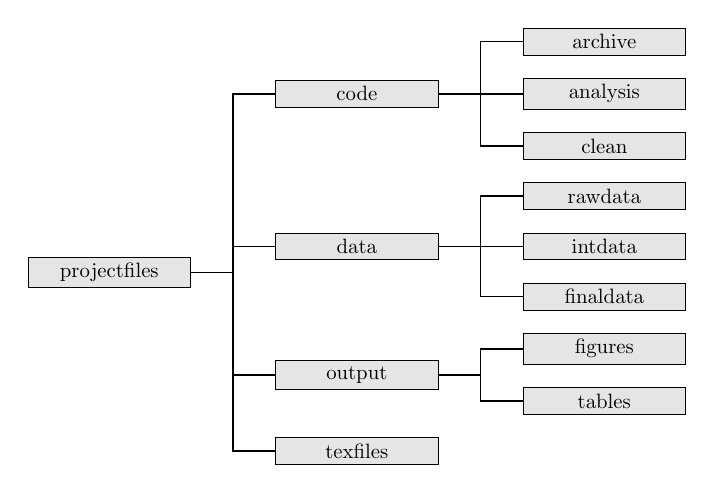
\begin{tikzpicture}[level distance=1.65in, sibling distance=.15in, scale=0.75]
            \tikzset{edge from parent/.style= {thick, draw, edge from parent fork right}, every tree node/.style={draw,minimum width=.15in, text width=1in, align=center, fill=gray!20, inner sep=3pt}, grow'=right}
                    \Tree 
                    [. {projectfiles} 
                        [.{code}
                            [.{archive} ]
                            [.{analysis} ]
                            [.{clean} ]
                        ]
                        [. {data}
                            [.{rawdata} ]
                            [.{intdata} ]
                            [.{finaldata} ]
                        ]
                        [.{output}
                            [.{figures} ]
                            [.{tables} ]
                        ]
                        [.{texfiles} ]
                        ]
            \end{tikzpicture}
            \vskip.2cm
            \item
            Include a \texttt{readme.txt} file in the main folder to explain the structure to other users.
		\end{itemize}
		\item[5.]
		\textbf{Automation}: If you want your code to repeat the same action, you should write it in a way that allows you to re-use the relevant chunk of code by calling it (do not copy-paste chunks of code!).
		\begin{itemize}
			\item
			Defining your own functions is very useful.
			\item
			Allows you to fix errors much faster by making changes only in one place.
			\vskip.6cm
		\end{itemize}
		\item
		More good practices: \textit{Code and Data for the Social Sciences: A Practitioner's Guide} (by Matt Gentzkow and Jesse Shapiro), 
		\vskip.2cm
		\scriptsize \url{http://web.stanford.edu/~gentzkow/research/CodeAndData.pdf}.
		\vskip.2cm
		\begin{itemize}
			\item
			This guide details best practices for managing research projects. You will certainly benefit from reading it in your own future projects or when doing RA work. It is mostly geared towards Stata users, but many of the principles apply to R users as well.
		\end{itemize}
	\end{itemize}
	
\end{frame}




\section[R]{Introduction to R}

\subsection{About R \& RStudio}

\begin{frame}[allowframebreaks]
 \frametitle{About R}

	\begin{itemize}
		\item
		R is a programming \textbf{language and environment} that is developed specifically for implementing statistical methods.
		\begin{itemize}
			\item
			It is designed for matrix handling, statistical analysis and data visualization.
			\item
			By contrast, Matlab was created with engineering applications in mind.
		\end{itemize}
		\item
		Importantly, R is \textbf{open source}, and it is used by most statisticians, which makes R highly responsive to new developments in methodology.
		\begin{itemize}
			\item
			There are thousands of free extension \textbf{packages} available online, and there is a large \textbf{community} of R users who are willing to share their knowledge and code.
			\item
			A (somewhat outdated) New York Times article on the growing popularity of R:
			
			\scriptsize \url{http://www.nytimes.com/2009/01/07/technology/business-computing/07program.html?pagewanted=1&_r=0}\small .
			\item
			By contrast, Stata and Matlab require paid licenses.
		\end{itemize}
		\item
		In my opinion, it's best to have at least basic knowledge of several programming languages, so that you can always choose the most appropriate tool for the task at hand... But if you are an economics major and you were going to learn only one language, then R is currently the best available option.
	\end{itemize}
	
	The R packages ecosystem:
		\begin{figure}
		\centering
		\includegraphics[width=.8\textwidth]{figures/rpackages_eco}
		\caption{\scriptsize The `Ecosystem of R packages': correlations are based on packages mentioned in Stack Overflow answers on the same question. This image is taken from \tiny\url{https://stackoverflow.blog/2017/10/10/impressive-growth-r}\scriptsize.}
		\label{Fig: 1}
		\end{figure}
	
	The R packages ecosystem:
		\begin{figure}
		\centering
		\includegraphics[width=.8\textwidth]{figures/rpackages_eco_cat}
		\caption{\scriptsize The `Ecosystem of R packages': correlations are based on packages mentioned in Stack Overflow answers on the same question. This image is taken from \tiny\url{https://stackoverflow.blog/2017/10/10/impressive-growth-r}\scriptsize.}
		\label{Fig: 1}
		\end{figure}
	
	The number of packages published on CRAN (=Comprehensive R Archive Network):
		\begin{figure}
		\centering
		\includegraphics[width=.75\textwidth]{figures/rpackages}
		\caption{\scriptsize Number of published R packages over time. This image is taken from \tiny\url{https://gist.github.com/daroczig/3cf06d6db4be2bbe3368}\scriptsize, which also contains an instructive example of R code for extracting data from web pages.}
		\label{Fig: 1}
		\end{figure}
	
	
	\begin{itemize}
		\item
		R vs. Python, what's the difference?
		\vskip.5cm
		\begin{columns}[t]
		\begin{column}{0.1\textwidth}
		\end{column}
		\begin{column}{0.4\textwidth}
		\hskip1cm R:
		\begin{itemize}
			\item[Intended users]
			%\vskip-.5cm
			Statisticians
			\item[Within econ]
			\vskip-.2cm
			Micro, metrics
			\item[Cost]
			\vskip-.2cm
			Free
		\end{itemize}
		\end{column}
		\begin{column}{0.5\textwidth}
		\hskip.5cm Python:
		\begin{itemize}
			\item[]
			%\vskip-.5cm
			General Purpose
			\item[]
			\vskip-.2cm
			Machine Learning, Macro
			\item[]
			\vskip-.2cm
			Free
		\end{itemize}
		\end{column}
		\end{columns}
		\vskip.5cm
		\item
		So what should you use?
		\begin{itemize}
			\item
			For small projects and simple tasks, it doesn't matter much.
			\item
			The choice between Matlab and Python (and Stata) becomes important when you're doing very specialized tasks; having a package or a toolbox available that implements the complicated estimation method you want to use could save you lots of time!
			\begin{itemize}
				\item
				To explore a data set, try out a recently developed machine learning technique, or do data analysis using methods not built into Stata $\rightarrow$ use R or Python.
				\item For projects involving more traditional econometrics, use R. For projects using newer methods, e.g. techniques within machine learning, Python might be a better choice.
				\item
				For projects involving more general purpose programming (e.g. web scraping), use Python.
			\end{itemize}
		\end{itemize}
	\end{itemize}
\end{frame}





\begin{frame}[allowframebreaks]
 \frametitle{RStudio}

	\begin{itemize}
		\item
		The standard, built-in R GUI looks like this:
		\begin{figure}
		\centering
		\includegraphics[width=.85\textwidth]{figures/fig1}
		\caption{\scriptsize R environment.}
		\label{Fig: 1}
		\end{figure}
		\item
		Rather than use the standard R environment as a graphical interface for R, I recommend that you use \textbf{RStudio}.
		\vskip.5cm
		\item
		Both R and RStudio can be downloaded for free and are available for Windows, Mac, and Linux/UNIX:
		\begin{itemize}
			\item
			Download R: \scriptsize \url{http://cran.r-project.org/}.\small
			\vskip.1cm
			\item
			Download RStudio Desktop: \scriptsize \url{https://www.rstudio.com/products/rstudio/}.\\
		\end{itemize}
		\vskip10cm
		\item
		The RStudio interface looks something like this:
		\begin{figure}[h!]
		\centering
		\includegraphics[scale = .2]{figures/RStudio1.png}
		\caption[]{RStudio.}
		\label{Fig: 2}
		\end{figure}
		\item[]
		\item
		You can change the interface (arrangement of the panels, color scheme, ..) by selecting `Tools' and then `Global Options' in the menu above.
		\vfill
		\item
		Let's try it out...
		\begin{itemize}
			\item
			Commands from the demonstration are in the file \textts{REU\_commands.R} on the website.
			\item
			Solutions to exercises are also in that file.
		    \vfill
		\end{itemize}
		
		\item
		A useful shortcut in RStudio is \textts{alt+shift+k}: it shows an overview of all shortcuts.
		
		\vskip.5cm
		
		\begin{myexc}[Simple calculations]
		Using the command line, compute the following:
		\begin{enumerate}[(a)]
			\item
			$\sqrt{e^{2}}$
			\item
			$\Phi(.5), \text{ where } \Phi(\cdot) \text{ is the standard Normal CDF}$ (\ul{Hint}: Look up the correct syntax for \textts{pnorm()} in the `Help' tab).
			\item
			$\max\{1,\left[\sin(\pi/2)\right]^2\}$
		\end{enumerate}
		\addtocounter{exccounter}{1}
		\end{myexc}
	\end{itemize}
	
\end{frame}





\subsection{Getting used to the R syntax: simple calculations, vectors, matrices}

\begin{frame}[allowframebreaks]
 \frametitle{Vectors and matrices}

	\begin{itemize}
		\item
		Before we go through a more challenging example, let's briefly practice working with vectors and matrices in R.
	\end{itemize}

	\begin{myexc}[Vectors]
	\fontsize{9pt}{12}\selectfont
	\begin{enumerate}[(a)]
		\item
		Define the vectors
		\vskip-.6cm
		\begin{align*}
			\texttt{x} = \begin{bmatrix}
				1 \\ 2\\ 3
			\end{bmatrix}, \qquad \texttt{y} = \begin{bmatrix}
				4 \\ 5 \\ 6
			\end{bmatrix}.
		\end{align*}
		Do this once using the $\texttt{c()}$ command and once using $\texttt{seq()}$. Also try \texttt{1:3}.
		\item
		What is the difference between \texttt{x*y} and \texttt{x\%*\%y}?
		\item
		Using $\texttt{x}$ and $\texttt{y}$ as in the previous exercise, try \texttt{cbind(x,y)} and \texttt{rbind(x,y)}.
		\item
		Using $\texttt{x}$ and $\texttt{y}$ as before, what is the difference between \texttt{max(x,y)}, \texttt{pmax(x,y)}, \texttt{apply(cbind(x,y),1,max)}, and \texttt{apply(cbind(x,y),2,max)}?
	\end{enumerate}
	\addtocounter{exccounter}{1}
	\end{myexc}
	
	\begin{itemize}
		\item
		\textbf{Indexing}: use square brackets to extract one or several elements of the vector.
		\begin{itemize}
			\item
			For example, \texttt{x[1]} extracts the first element of vector \texttt{x}.
		\end{itemize}
	\end{itemize}
	
	\begin{myexc}[Vectors, continued]
	\fontsize{9pt}{12}\selectfont
	Define $\texttt{x} = \begin{bmatrix}
		1 & 2 & 3 & 4 & 5 & 6
	\end{bmatrix}$.
	\begin{enumerate}[(a)]
		\item
		Sum all the elements.
		\item
		Calculate the mean.
		\item
		Replace the first element by 0.
		\item
		Add 1 to all elements and save the result in a vector \texttt{y}.
		\item
		What is the result of \texttt{x[c(1,3)]}? \texttt{x[2:4]}? \texttt{x[-2]}? \texttt{x[x<4]}?
		\item
		Add 1 to the first, third, and fifth element of \texttt{x}. (Using a single statement).
		\item
		Add 1 to all elements of \texttt{x} with a value strictly less than 4. (Using a single statement).
		\item
		What happens if we type \texttt{x[7] <- 7}? And \texttt{x[9] <- 9}?
	\end{enumerate}
	\addtocounter{exccounter}{1}
	\end{myexc}
	
	\vskip2cm
	
	\begin{myexc}[Matrices]
	\fontsize{9pt}{12}\selectfont
	Create the following matrices:
	\begin{align*}
		\texttt{A} = \begin{bmatrix}
		 	1 & 2 & 3 \\
		 	1 & 2 & 3 \\
		 	1 & 2 & 3 
			\end{bmatrix}, \qquad \texttt{B} = \begin{bmatrix}
			4 & 0 & 0 \\
			0 & 5 & 0 \\
			0 & 0 & 6 
		\end{bmatrix}.
	\end{align*}
	To create $A$, use the command \texttt{matrix()}. To create $B$, use the command \texttt{diag()}.
	\begin{enumerate}[(a)]
		\item
		What is the difference between \texttt{A*B} and \texttt{A\%*\%B}?
		\item
		What does \texttt{A[1,]} do? And \texttt{A[,1]}?
		\item
		What does \texttt{t(A)} do? And \texttt{solve(A)}? Why doesn't this command work? Does it work on $\texttt{B}$?
		\item
		Replace the $(2,2)$ element of $\texttt{A}$ by 1.
		\item
		Replace the diagonal of $\texttt{A}$ by ones.
		\item
		Store the first two rows of \texttt{A} in a new matrix $\texttt{C}$ (so that \texttt{C} is a $2\times 3$ matrix).
		\item
		What does \texttt{dim(C)} do? And \texttt{nrow(C)}?
	\end{enumerate}
	\addtocounter{exccounter}{1}
	\end{myexc}



%	\begin{myexm}[Test example]
%		\fontsize{9pt}{12}\selectfont
%		Blabla
%		<<sererter,fig.width=5,fig.height=3.2,out.width='.45\\linewidth',size="scriptsize",echo=TRUE>>=
%		set.seed(209); N <- 1000
%
%		wages <- rlnorm(N); employment.status <- ( wages + rnorm(N) > 0 )
%
%		hist(wages, n=100, xlim=c(0,7), ylim=c(0,200))
%
%		hist(employment.status*wages, n=100, xlim=c(0,7), ylim=c(0,200))
%		@
%	\addtocounter{exmcounter}{1}
%	\vskip-.2cm
%	\end{myexm}
	
\end{frame}



%\subsection{Example: numerical integration}

\begin{frame}[allowframebreaks]
 \frametitle{Example: numerical integration}

	\begin{itemize}
		\item
		Let's go over some basic R commands by walking through a longer example. We'll try to approximate an integral.
		\item
		Recall the example of calculating $\pi$ by throwing darts at a board. Suppose
		we take draws from a distribution uniformly distributed over the unit square 
		$[0,1] \times [0,1]$. Take $N$ draws. Calculate the fraction of draws that land
		within the circle with center at the origin and radius equal to one: 
		$y^2 + x^2 = 1$. 
		This is 
		equivalent to computing the integral
		$$		
		\int_0^1 \sqrt[+]{1 - x^2} \mathrm d x.
		$$
		\item
		We don't want to calculate the integral analytically. Instead, we can use \textit{simulation} to approximate it.
		\begin{itemize}
			\item
			In R, it is easy to generate `pseudo-random' values, and to evaluate the function $\phi(x)$.
		\end{itemize}
		\item
		The idea is to ``throw darts" at a rectangle of known area that encloses the area under the graph. In R, we can easily assess what fraction of the darts has landed in the area that we want to approximate (the fraction that has landed below the PDF), and take this fraction of the total known area as our approximation.
		\begin{figure}
		\centering
		\includegraphics[width=.55\textwidth]{figures/fig3}
		\caption{\scriptsize Numerical integration example.}
		\label{Fig: 1}
		\end{figure}
		\item
		The code is in the file \texttt{\scriptsize REU\_integration.R}.
	\end{itemize}
	
\end{frame}




\subsection{Functions}

\begin{frame}[allowframebreaks]
 \frametitle{Functions}

	\begin{itemize}
		\item
		Suppose that we want to re-use the code from the previous example to repeatedly approximate 
		$$		
		\int_0^1 4 \sqrt[+]{1 - x^2} \mathrm d x.
		$$
		for some user-specified value of $N$. Then it is convenient to write a function that takes as input the \textbf{parameter} $N$.
		\item
		The syntax for defining a function is
		\begin{align*}
			\texttt{<FunName> <- } & \texttt{\alert{function}(<par1>,<par2>) } \texttt{\{} \\
			& \qquad \texttt{<...commands...>} \\
			& \qquad \texttt{\alert{return}(<output>)} \\
			&\texttt{\}}			
		\end{align*}
		\item
		The code in the file \texttt{\scriptsize REU\_function.R} defines such a function, building on the numerical integration example.
		\item
		You can copy-paste the contents of this file to the command line, or you can save the file as an \texttt{.R} file in your working directory so that it can be sourced from the command line by typing
		\begin{align*}
			\texttt{source("REU\_function.R")}.
		\end{align*}
		\item
		After sourcing this code (look for \texttt{NumInt} in the workspace to see if this was successful), we are able to call the function from the command line, or from another \texttt{.R} file.
		\begin{itemize}
			\item
			E.g., type \texttt{NumInt(1000)} on the command line.
		\end{itemize}
		\vskip4cm
		\item
		Things to notice in the function code:
		\begin{itemize}
			\item
			It is good practice to include \textbf{error handling}. For example, the user might specify $N > 0$, for which this code will return the error message that we specified.
			\item
			\textbf{Comments} add structure, make it easy to read the code.
			\item
			R suppresses \textbf{intermediate output} in a function. Using \texttt{print()} for printing intermediate output in a function can help you when testing/debugging your code.
			\item
			An \texttt{if} statement was used for handling errors. The syntax for such a statement is:
			\vskip-.5cm
			\begin{align*}
				\texttt{\alert{if}(<logical statement>) } & \texttt{\{} \\
				& \qquad \texttt{<...commands...>} \\
				&\texttt{\}}			
			\end{align*}
			\begin{itemize}
				\item
				\vskip-.4cm
				A logical statement can be either true or false. In our example, \texttt{N > 0}.
				\item
				We can combine logical statements, using
				\vskip-.5cm
				\begin{align*}
					&\texttt{<logical statement1>} \texttt{ \alert{\&} } \texttt{<logical statement2>}\\
					&\texttt{<logical statement1>} \texttt{ \alert{|} } \texttt{<logical statement2>}
				\end{align*}
			\end{itemize}
		\end{itemize}
	\end{itemize}

	\begin{myexc}[Logical statements]
	\fontsize{9pt}{12}\selectfont
		Using the command line, type
		\begin{align*}
			\texttt{a <- 1}; \tab \texttt{b <- 0}.
		\end{align*}
		Which relationships are tested by the following commands?
		\begin{enumerate}[(a)]
			\item
			\texttt{ a == b }
			\item
			\texttt{ a >= b }
			\item
			\texttt{ a < 0 }
			\item
			\texttt{ a != b }
			\item
			\texttt{ a | b }
			\item
			\texttt{ a \& b }
			\item
			\texttt{ !a }
		\end{enumerate}
	\addtocounter{exccounter}{1}
	\end{myexc}
	
\end{frame}



\subsection{Control statements: if, for, while}

\begin{frame}[allowframebreaks]
 \frametitle{Control statements: if, for, while}

	\begin{itemize}
		\item
		A control statement is a statement that determines whether other statements will be executed.
		\begin{itemize}
			\item
			We just saw the syntax for an \texttt{if} statement. If the logical statement inside parentheses is true, the commands between the curly braces are executed.
			\item
			We will see two other examples: \texttt{for} loops and \texttt{while} loops.
		\end{itemize}
		\item
		\texttt{for} loop syntax:
		\vskip-.7cm
		\begin{align*}
			\texttt{\alert{for}(i in seq) } & \texttt{\{} \\
			& \qquad \texttt{<...commands...>} \\
			&\texttt{\}}			
		\end{align*}
		\vskip-.4cm
		\scriptsize \texttt{seq} stores the values that \texttt{i} can take. It is usually a range of consecutive integers,  but it can also be a set of strings.
		\item
		\normalsize
		\texttt{while} loop syntax:
		\vskip-.6cm
		\begin{align*}
			\texttt{\alert{while}(<logical statement>) } & \texttt{\{} \\
			& \qquad \texttt{<...commands...>} \\
			&\texttt{\}}			
		\end{align*}
		\item
		The code in \texttt{\scriptsize REU\_control.R} simulates a data set using a \texttt{for} loop. The data-generating process is
		\begin{align*}
			Y_i = a + b X_i + \varepsilon_i, \qquad i=1,..,N,
		\end{align*}
		where $X_i\sim(3,1)$, $\varepsilon_i\sim(0,1)$, $a=2$ and $b=.5$, $N=200$.
		\begin{itemize}
			\item
			Data is simulated for $X_i$ and $\varepsilon_i$, $i=1,..,N$, and stored in vectors
			\begin{align*}
				\texttt{X} = \begin{bmatrix}
					X_1 & \cdots & X_N
				\end{bmatrix}'; \texttt{E} = \begin{bmatrix}
					\varepsilon_1 & \cdots & \varepsilon_N
				\end{bmatrix}'.
			\end{align*}
			\item
			We can use a \texttt{for} loop to generate the $Y_i$ values. We first generate a vector of NA's (NA stands for``Not Available"), and then we `walk through' the vector using a \textbf{counter} or \textbf{index} \texttt{i}. In every step of the loop, we replace the NA by a value.
			\begin{itemize}
				\item
				At the end of each step, the counter is automatically updated.
			\end{itemize}
			\vskip3cm
			\item
			This is not the fastest way to generate the simulated data... It would have been faster to just write
			\vskip-.7cm
			\begin{align*}
				\texttt{Y <- a + X * b + E}
			\end{align*}
			\begin{itemize}
				\item
				\vskip-.7cm
				Note that R adapts to the object it is asked to work on: R understands the $+$ and $*$ operations as operations on vectors rather than scalars.
				\item
				This is both an advantage and a disadvantage of R: sometimes it's convenient, and sometimes it produces unexpected output. You should always check whether R is doing what you want it to do when vectors and matrices are involved.
				\item
				For example, when you add two vectors of unequal length, R will recycle elements of the shorter vector to match the longest vector, and this may not be what you want. Matlab would give you an error message.
			\end{itemize}
		\end{itemize}
		\item
		A \texttt{while} loop can be used to do the exact same thing as the \texttt{for} loop from the previous example. Things to pay attention to in the code:
		\begin{itemize}
			\item
			A \texttt{while} loop can have more flexible stopping criteria than a \texttt{for} loop. But you should make sure the stopping criterion will be satisfied before you run out of memory...
			\item
			The counter is not automatically updated. To update in every step, `self referencing' is used: \texttt{i <- i+1} adds 1 to \texttt{i}.
		\end{itemize}
	\end{itemize}
	
\end{frame}





\subsection{Regression}

\begin{frame}[allowframebreaks]
 \frametitle{Regression}

	\begin{itemize}
		\item
		We can use the data that we have just simulated to run a regression.
		\begin{itemize}
			\item
			The syntax for \textbf{simple regression} is
			\begin{align*}
				\texttt{<output.name> <- \alert{lm}(Y $\sim$ X, data = <data.name>)} 
			\end{align*}
			\item
			The syntax for \textbf{multiple regression} is
			\begin{align*}
				\texttt{<output.name> <- \alert{lm}(Y $\sim$ X1 + X2, data = <data.name>)} 
			\end{align*}
			\item
			These statements produce objects that can be read by \texttt{summary()} to produce a quick overview of the regression results in RStudio.
			\item
			You will often want to produce \textbf{LaTeX tables}. Two packages that will be useful are \texttt{xtable} and \texttt{stargazer}.
			\item
			A demonstration of how to produce summary statistics, load and save data, and running regressions is in \texttt{\scriptsize REU\_regression.R}.
		\end{itemize}
		\item[]
		\begin{table}[ht]
		\centering \scriptsize
		  \caption{Produced with the \texttt{xtable} package.}
		  \label{}
		\begin{tabular}{rrrrr}
		  \hline
		 & Estimate & Std. Error & t value & Pr($>$ $|$t$|$) \\ 
		  \hline
		(Intercept) & 1.5505 & 0.2027 & 7.65 & 0.0000 \\ 
		  X & 0.6421 & 0.0632 & 10.16 & 0.0000 \\ 
		   \hline
		\end{tabular}
		\end{table}
		\vskip8cm
		\item[]
		\begin{table}[!htbp] \centering  \scriptsize
		  \caption{Produced with the \texttt{stargazer} package.} 
		  \label{} 
		\begin{tabular}{@{\extracolsep{5pt}}lc} 
		\\[-1.8ex]\hline 
		\hline \\[-1.8ex] 
		 & \multicolumn{1}{c}{\textit{Dependent variable:}} \\ 
		\cline{2-2} 
		\\[-1.8ex] & Y \\ 
		\hline \\[-1.8ex] 
		 X & 0.642$^{***}$ \\ 
		  & (0.063) \\ 
		  & \\ 
		 Constant & 1.550$^{***}$ \\ 
		  & (0.203) \\ 
		  & \\ 
		\hline \\[-1.8ex] 
		Observations & 200 \\ 
		R$^{2}$ & 0.343 \\ 
		Adjusted R$^{2}$ & 0.339 \\ 
		Residual Std. Error & 0.906 (df = 198) \\ 
		F Statistic & 103.218$^{***}$ (df = 1; 198) \\ 
		\hline 
		\hline \\[-1.8ex] 
		\textit{Note:}  & \multicolumn{1}{r}{$^{*}$p$<$0.1; $^{**}$p$<$0.05; $^{***}$p$<$0.01} \\ 
		\end{tabular}
		\end{table}
		\vskip2cm
		\item[]
		\begin{table}[!htbp] \centering \tiny
  		\caption{Produced with the \texttt{stargazer} package, incorporating output from two regression specifications.} 
 		 \label{} 
		\begin{tabular}{@{\extracolsep{5pt}}lcc} 
		\\[-1.8ex]\hline 
		\hline \\[-1.8ex] 
		 & \multicolumn{2}{c}{\textit{Dependent variable:}} \\ 
		\cline{2-3} 
		\\[-1.8ex] & \multicolumn{2}{c}{Y} \\ 
		\\[-1.8ex] & (1) & (2)\\ 
		\hline \\[-1.8ex] 
		 X & 0.642$^{***}$ & 0.639$^{***}$ \\ 
		  & (0.063) & (0.063) \\ 
		  & & \\ 
		 Z &  & 0.084 \\ 
		  &  & (0.065) \\ 
		  & & \\ 
		 Constant & 1.550$^{***}$ & 1.385$^{***}$ \\ 
		  & (0.203) & (0.240) \\ 
		  & & \\ 
		\hline \\[-1.8ex] 
		Observations & 200 & 200 \\ 
		R$^{2}$ & 0.343 & 0.348 \\ 
		Adjusted R$^{2}$ & 0.339 & 0.342 \\ 
		Residual Std. Error & 0.906 (df = 198) & 0.904 (df = 197) \\ 
		F Statistic & 103.218$^{***}$ (df = 1; 198) & 52.602$^{***}$ (df = 2; 197) \\ 
		\hline 
		\hline \\[-1.8ex] 
		\textit{Note:}  & \multicolumn{2}{r}{$^{*}$p$<$0.1; $^{**}$p$<$0.05; $^{***}$p$<$0.01} \\ 
		\end{tabular} 
		\end{table} 
	\end{itemize}
	
\end{frame}










\section[Matlab]{Comparison with Matlab}


\subsection{Syntax: differences between R and Matlab}

\begin{frame}[allowframebreaks]
 \frametitle{Syntax: differences between R and Matlab}
 
 	\begin{itemize}
 		\item
 		The table below is based on David Hiebeler's Matlab/R reference, which you can find here: \scriptsize \url{http://www.math.umaine.edu/~hiebeler/comp/matlabR.pdf}.
 	\end{itemize}

		\vskip-.5cm
		\begin{columns}[t]
		\fontsize{8pt}{11}\selectfont
		\begin{column}{0.1\textwidth}
		\end{column}
		\begin{column}{0.4\textwidth}
		\hskip1cm R:
		\begin{itemize}
%			\item[Help]
%			\texttt{help(sqrt)}
			\item[Computations]
			\vskip-.2cm
			\texttt{a+b, a-b, a*b, a/b}
			\item[]
			\vskip-.2cm
			\texttt{sqrt(a), exp(a), sin(a)}
			\item[]
			\vskip-.2cm
			\texttt{a\^}\texttt{b}
			\item[]
			\vskip-.2cm
			\texttt{a\&b, a|b, a==b, a!=b}
			\item[Vectors]
			\vskip-.2cm
			\texttt{x <- c(1,2,3)}
			\item[]
			\vskip-.2cm
			
			\item[]
			\vskip-.2cm
			\texttt{x[2]}
			\item[]
			\vskip-.2cm
			\texttt{x[2:length(x)]}
			\item[]
			\vskip-.2cm
			\texttt{x[1:length(x)-1]}
			\item[]
			\vskip-.2cm
			\texttt{1:6}
			\item[]
			\vskip-.2cm
			\texttt{seq(1,6,by=2)}
			\item[]
			\vskip-.2cm
			\texttt{seq(1,6,len=100)}
			\item[]
			\vskip-.2cm
			\texttt{t(x)}
			\item[Matrices]
			\vskip-.2cm
			\texttt{A <- matrix(1:6, nrow=2)}
			\item[]
			\vskip-.2cm
			\texttt{A[1,2]}
			\item[]
			\vskip-.2cm
			\texttt{A[1,]}
			\item[]
			\vskip-.2cm
			\texttt{cbind(x,y)}
			\item[]
			\vskip-.2cm
			\texttt{rbind(x,y)}
			\item[]
			\vskip-.2cm
			\texttt{A \%*\% B}
			\item[]
			\vskip-.2cm
			\texttt{A * B}
			\item[]
			\vskip-.2cm
			\texttt{solve(A), det(A)}
			\item[]
			\vskip-.2cm
			\texttt{solve(A,b)}
			\item[]
			\vskip-.2cm
			\texttt{mean(A)}
			\item[]
			\vskip-.2cm
			\texttt{colMeans(A), rowMeans(A)}
		\end{itemize}
		\end{column}
		\begin{column}{0.5\textwidth}
		\hskip1cm Matlab:
		\begin{itemize}
%			\item[]
%			\texttt{help sqrt}
			\item[]
			\vskip-.2cm
			\texttt{a+b, a-b, a*b, a/b}
			\item[]
			\vskip-.2cm
			\texttt{sqrt(a), exp(a), sin(a)}
			\item[]
			\vskip-.2cm
			\texttt{a\^}\texttt{b}
			\item[]
			\vskip-.2cm
			\texttt{a\&b, a|b, a==b, a$\scriptsize \sim$=b}
			\item[]
			\vskip-.2cm
			\texttt{x = [1 2 3]} (row vector)
			\item[]
			\vskip-.2cm
			\texttt{x = [1; 2; 3]} (column vector) {\color{beamer@myRed} $\leftarrow$ !}
			\item[]
			\vskip-.2cm
			\texttt{x(2)}
			\item[]
			\vskip-.2cm
			\texttt{x(2:end)}
			\item[]
			\vskip-.2cm
			\texttt{x(1:end-1)}
			\item[]
			\vskip-.2cm
			\texttt{1:6}
			\item[]
			\vskip-.2cm
			\texttt{1:2:6}
			\item[]
			\vskip-.2cm
			\texttt{linspace(1,6,100)}
			\item[]
			\vskip-.2cm
			\texttt{x'}
			\item[]
			\vskip-.2cm
			\texttt{A = [1 3 5; 2 4 6]} {\color{beamer@myRed} $\leftarrow$ !}
			\item[]
			\vskip-.2cm
			\texttt{A(1,2)}
			\item[]
			\vskip-.2cm
			\texttt{A(1,:)}
			\item[]
			\vskip-.2cm
			\texttt{[x y]}
			\item[]
			\vskip-.2cm
			\texttt{[x; y]}
			\item[]
			\vskip-.2cm
			\texttt{A*B}
			\item[]
			\vskip-.2cm
			\texttt{A.*B}
			\item[]
			\vskip-.2cm
			\texttt{inv(A), det(A)}
			\item[]
			\vskip-.2cm
			\texttt{A $\backslash$ b} {\color{beamer@myRed} $\leftarrow$ !}
			\item[]
			\vskip-.2cm
			\texttt{mean(A(:))}
			\item[]
			\vskip-.2cm
			\texttt{mean(A), mean(A,2)}
		\end{itemize}
		\end{column}
		\end{columns}
		
		
		
		\begin{myexc}[System of linear equations]
		\fontsize{9pt}{11}\selectfont
		Solve the following system of linear equations, using Matlab:
		\begin{align*}
			x_1 + 2 x_2 - 2x_2 &= 1 \\
			3 x_1 + 5 x_2 + 6 x_3 &= 2 \\
			7 x_1 + 8 x_2 + 9 x_3 &= 3 
		\end{align*}
		\underline{Hint}: Recall \texttt{A $\backslash$ b} from the previous slide.
		\addtocounter{exccounter}{1}
		\end{myexc}
%		
%		\begin{myexc}[Vectors and matrices]
%		\fontsize{9pt}{11}\selectfont
%		Attempt the exercises for vectors and matrices in R, using Matlab.
%		\addtocounter{exccounter}{1}
%		\end{myexc}
%		
		
		\vskip6cm
		
		\begin{columns}[t]
		\fontsize{7pt}{9}\selectfont
		\begin{column}{0.05\textwidth}
		\end{column}
		\begin{column}{0.45\textwidth}
		\hskip1cm R:
		\begin{itemize}
			\item[if] \text{ }
			\vskip-1cm
			\begin{flalign*}
				& \texttt{\alert{if}(<logical statement>) } \texttt{\{} &\\
				& \qquad \texttt{<...commands...>} &\\
				& \texttt{\}}			
			\end{flalign*}
			\item[if/else] \text{ }
			\vskip-1cm
			\begin{flalign*}
				& \texttt{\alert{if}(<logical statement>) } \texttt{\{} &\\
				& \qquad \texttt{<...commands...>} &\\
				& \texttt{\}} \texttt{\alert{ else }} \texttt{\{} &\\
				& \qquad \texttt{<...commands...>} &\\
				& \texttt{\}}
			\end{flalign*}
			\item[for] \text{ }
			\vskip-1cm
			\begin{flalign*}
				& \texttt{\alert{for}(i in seq) } \texttt{\{} &\\
				& \qquad \texttt{<...commands...>} &\\
				& \texttt{\}}			
			\end{flalign*}
			\item[while] \text{ }
			\vskip-1cm
			\begin{flalign*}
				& \texttt{\alert{while}(<logical statement>) } \texttt{\{} &\\
				& \qquad \texttt{<...commands...>} &\\
				& \texttt{\}}			
			\end{flalign*}
		\end{itemize}
		\end{column}
		\begin{column}{0.5\textwidth}
		\hskip1cm Matlab:
		\begin{itemize}
			\item[] \vskip-0.7cm
			\begin{flalign*}
				& \texttt{\alert{if} <logical statement> } &\\
				& \qquad \texttt{<...commands...>} &\\
				& \texttt{\alert{end}}&
			\end{flalign*}
			\item[] \vskip-0.7cm
			\begin{flalign*}
				& \texttt{\alert{if} <logical statement> } &\\
				& \qquad \texttt{<...commands...>} &\\
				& \texttt{\alert{else}} &\\
				& \qquad \texttt{<...commands...>} &\\
				& \texttt{\alert{end}}
			\end{flalign*}
			\item[] \vskip-0.7cm
			\begin{flalign*}
				& \texttt{\alert{for} i=seq} &\\
				& \qquad \texttt{<...commands...>} &\\
				& \texttt{\alert{end}}
			\end{flalign*}
			\item[] \vskip-0.7cm
			\begin{flalign*}
				& \texttt{\alert{while} (<logical statement>) } &\\
				& \qquad \texttt{<...commands...>} &\\
				& \texttt{\alert{end}}
			\end{flalign*}
		\end{itemize}
		\end{column}
		\end{columns}


		\begin{columns}[t]
		\fontsize{7pt}{9}\selectfont
		\begin{column}{0.05\textwidth}
		\end{column}
		\begin{column}{0.45\textwidth}
		\hskip1cm R:
		\begin{itemize}
			\item[function] \text{ }
			\vskip-1cm
			\begin{flalign*}
			& \texttt{<FnName> <- } \texttt{\alert{function}(<x1>,<x2>) } \texttt{\{} &\\
			& \qquad \texttt{<...commands...>} &\\
			& \qquad \texttt{\alert{return}(<output>)} &\\
			& \texttt{\}}			
			\end{flalign*}
		\end{itemize}
		\end{column}
		\begin{column}{0.5\textwidth}
		\hskip1cm Matlab:
		\begin{itemize}
			\item[] \vskip-0.7cm
			\begin{flalign*}
				& \texttt{\alert{function} out.name=<FnName>(<x1>,<x2>)}  &\\
				& \qquad \texttt{<...commands...>} &\\
				& \texttt{out.name = <output>}
			\end{flalign*}
		\end{itemize}
		\end{column}
		\end{columns}
	
		
		Returning multiple values, objects that may have different types:
		\begin{columns}[t]
		\fontsize{7pt}{9}\selectfont
		\begin{column}{0.05\textwidth}
		\end{column}
		\begin{column}{0.45\textwidth}
		\hskip1cm R:
		\begin{itemize}
			\item[function] \text{ }
			\vskip-1cm
			\begin{flalign*}
				& \texttt{<FnName> <- } \texttt{\alert{function}(<x1>,<x2>) } \texttt{\{} &\\
			& \qquad \texttt{<...commands...>} &\\
			& \qquad \texttt{\alert{return}(list(<out1>,<out2>))} &\\
			& \texttt{\}}
			\end{flalign*}
		\end{itemize}
		\end{column}
		\begin{column}{0.5\textwidth}
		\hskip1cm Matlab:
		\begin{itemize}
			\item[] \vskip-0.7cm
			\begin{flalign*}
				& \texttt{\alert{function} [o1, o2]=<FnName>(<x1>,<x2>)}  &\\
				& \qquad \texttt{<...commands...>} &\\
				& \texttt{[o1, o2] = [<out1>, <out2>]}
			\end{flalign*}
		\end{itemize}
		\end{column}
		\end{columns}


\end{frame}







%\section[LaTeX]{Introduction to LaTeX}
%
%\subsection{LaTeX editor options}
%
%\begin{frame}[allowframebreaks]
% \frametitle{LaTeX editor options}
% 
% 	\begin{itemize}
%		\item
%		
%	\end{itemize}
%	
%\end{frame}
%

%Style files

%\subsection{Beamer}
%
%\begin{frame}[allowframebreaks]
% \frametitle{Beamer}
% 
% 	\begin{itemize}
%		\item
%		
%	\end{itemize}
%	
%\end{frame}





\section{Recommended resources}

\begin{frame}[allowframebreaks]
 \frametitle{Recommended resources}

 \textbf{R:}
 \begin{thebibliography}{10}

 \beamertemplatebookbibitems
 
 \bibitem{RIntroCore}
 W.N. Venables, D.M. Smith and the R Core Team - An Introduction to R
 \newblock{}
 \newblock{2017 version}
 \newblock{\scriptsize \url{http://cran.r-project.org/doc/manuals/R-intro.pdf}}

% \bibitem{StockWatson}
% J.H.~Stock \& M.W. Watson (3rd ed)
% \newblock {\em Introduction to Econometrics: Chapter 1, Sections 2.1-2.4, and Appendices 17.1, 17.2, 18.2.}

 \beamertemplateonlinebibitems
 
 \bibitem{RStudioTips}
 RStudio: Tips for learning R
 %\newblock{\em }
 \newblock{\scriptsize \url{http://www.rstudio.com/online-learning/}}
 
 \bibitem{GoogleRStyle}
 Google's R Style Guide
 %\newblock{\em }
 \newblock{\scriptsize \url{https://google.github.io/styleguide/Rguide.xml}}
 
 \bibitem{tidyverseRStyle}
 The tidyverse style guide
 %\newblock{\em }
 \newblock{\scriptsize \url{http://style.tidyverse.org/index.html}}

 \bibitem{tryr}
 TryR
 \newblock{}
 \newblock{Online interactive tutorial for first steps in R}
 \newblock{\scriptsize \url{http://tryr.codeschool.com/}}
 
 \bibitem{Forums}
 Stack Overflow, Cross Validated
 \newblock{}
 \newblock{Forums for programming and statistics questions}
 \newblock{\scriptsize \url{http://stackoverflow.com/}} and {\scriptsize \url{http://stats.stackexchange.com/}}
 
 \bibitem{MacR}
 Google Developers' Intro to R
 \newblock{}
 \newblock{Youtube tutorial videos -- geared towards Mac users}
 \newblock{\scriptsize \url{http://www.youtube.com/playlist?list=PLOU2XLYxmsIK9qQfztXeybpHvru-TrqAP}}
 
 \bibitem{HW}
 Hadley Wickham - Advanced R
 \newblock{}
 \newblock{Companion website for Advanced R book}
 \newblock{\scriptsize \url{http://adv-r.had.co.nz/}}
 
 \bibitem{GGHW}
 Garrett Grolemund \& Hadley Wickham - R for Data Science
 \newblock{}
 \newblock{Companion website for R for Data Science book}
 \newblock{\scriptsize \url{http://r4ds.had.co.nz/}}
 
 \bibitem{TS}
 Tom Short - R Reference Card
 \newblock{}
 \newblock{A useful cheat sheet, though somewhat outdated}
 \newblock{\scriptsize \url{http://cran.r-project.org/doc/contrib/Short-refcard.pdf}}
 
 \bibitem{TS}
 Knitr page, by Yihui Xie
 \newblock{}
 \newblock{Instructions for installing and using Knitr, a tool for integrating R code into LaTeX documents}
 \newblock{\scriptsize \url{http://yihui.name/knitr/}}

 
 \end{thebibliography}
 


 \vskip4cm
 \textbf{Matlab:}\\
 \begin{thebibliography}{10}
 
 \beamertemplateonlinebibitems
 
 \bibitem{MW}
 MathWorks video tutorials
 %\newblock{}
 %\newblock{Instructions for installing and using Knitr, a tool for integrating R code into LaTeX documents}
 \newblock{\scriptsize \url{http://www.mathworks.com/support/learn-with-matlab-tutorials.html?requestedDomain=www.mathworks.com}}

 \bibitem{Hiebeler}
 David Hiebeler - MATLAB / R Reference
 %\newblock{}
 \newblock{\scriptsize \url{http://www.math.umaine.edu/~hiebeler/comp/matlabR.pdf}}

 \beamertemplatebookbibitems

 \bibitem{LeSage}
 James P. LeSage - Applied Econometrics using MATLAB
 %\newblock{}
 \newblock{\scriptsize \url{http://www.spatial-econometrics.com/html/mbook.pdf}}

 \end{thebibliography}
 


 %\vskip4cm
 %\textbf{LaTeX:}\\
 %\begin{thebibliography}{10}

 %\beamertemplatearticlebibitems
 
 %\beamertemplateonlinebibitems

 %\bibitem{ShareLatex}
 %ShareLaTeX `Learn LaTeX in 30 minutes'
 %%\newblock{}
 %\newblock{\scriptsize \url{https://www.sharelatex.com/learn/Learn_LaTeX_in_30_minutes}}
 
 %\bibitem{TexGmail}
 %TeX for gmail
 %\newblock{}
 %\newblock{Add LaTeX capability to Gmail}
 %\newblock{\scriptsize \url{http://alexeev.org/gmailtex.html}}
 
 %\bibitem{Detexify}
 %Detexify
 %\newblock{}
 %\newblock{Recognizes handwritten symbols and returns suggestions for LaTeX code}
 %\newblock{\scriptsize \url{http://detexify.kirelabs.org/classify.html}}
 
 %\bibitem{TexStack}
 %LaTeX Stack Exchange
 %\newblock{}
 %\newblock{Forum for questions and answers about LaTeX syntax}
 %\newblock{\scriptsize \url{https://tex.stackexchange.com/}}
 
 %\bibitem{Texwikibook}
 %The LaTeX wikibook
 %\newblock{}
 %\newblock{In particular, consult the chapter on installation if you don't choose to work with LyX or ShareLaTeX}
 %\newblock{\scriptsize \url{https://en.wikibooks.org/wiki/LaTeX}}
 
 %\bibitem{ComparisonEditors}
 %A comparison of TeX editors (Wikipedia)
 %\newblock{}
 %\newblock{Use this to choose an editor if you don’t want to use LyX or ShareLaTeX -- I use and recommend Texmaker}
 %\newblock{\scriptsize \url{https://en.wikipedia.org/wiki/Comparison_of_TeX_editors}}

 %\end{thebibliography}

\end{frame}



\end{document}